\documentclass[11pt]{article}
\usepackage[margin=1in]{geometry}
\usepackage{amsmath, amssymb, amsthm}
\usepackage{physics}
\usepackage{bm}
\usepackage{hyperref}
\usepackage{graphicx}
\usepackage{enumitem}
\usepackage{siunitx}
\usepackage{mathtools}
\usepackage{braket}
\usepackage{quantikz}
\usepackage{tikz}
\usetikzlibrary{arrows.meta,calc}
\usepackage{MnSymbol,wasysym} % contains \smiley{}

\newenvironment{summary}{\par\noindent\textbf{Summary.} }{\par}

\title{CSCI-739 Quantum Machine Learning \\[4pt] \large Homework 5}
\date{}

\begin{document}
\maketitle

\begin{center}

This bonus homework is unlike the earlier ones. Instead of implementing algorithms or running simulations, 
you will explore a curated set of research papers spanning several themes in quantum computing that I 
personally enjoy thinking about and working on: quantum approaches to combinatorial optimization, 
quantum algorithms for applied mathematics and numerical PDEs, high-fidelity qubit control for more 
robust computation, and a new algorithmic framework called Decoded Quantum Interferometry (DQI). 

Each paper represents a different facet of how quantum computation may ultimately reshape optimization, 
scientific computing, control theory, and algorithm design. Your job is simply to read, reflect, and 
summarize—this homework is about intellectual curiosity, not coding. \smiley{}

If you are interested in pursuing a quantum computing–based capstone, or an unpaid research opportunity 
with me at RIT, please feel free to reach out. This assignment is meant to give you a preview of the 
directions I actively think about and where future student research projects can meaningfully contribute. \smiley{}

\end{center}
Also here is a meme:
\begin{figure}[h!]
\centering
\vspace{1em}
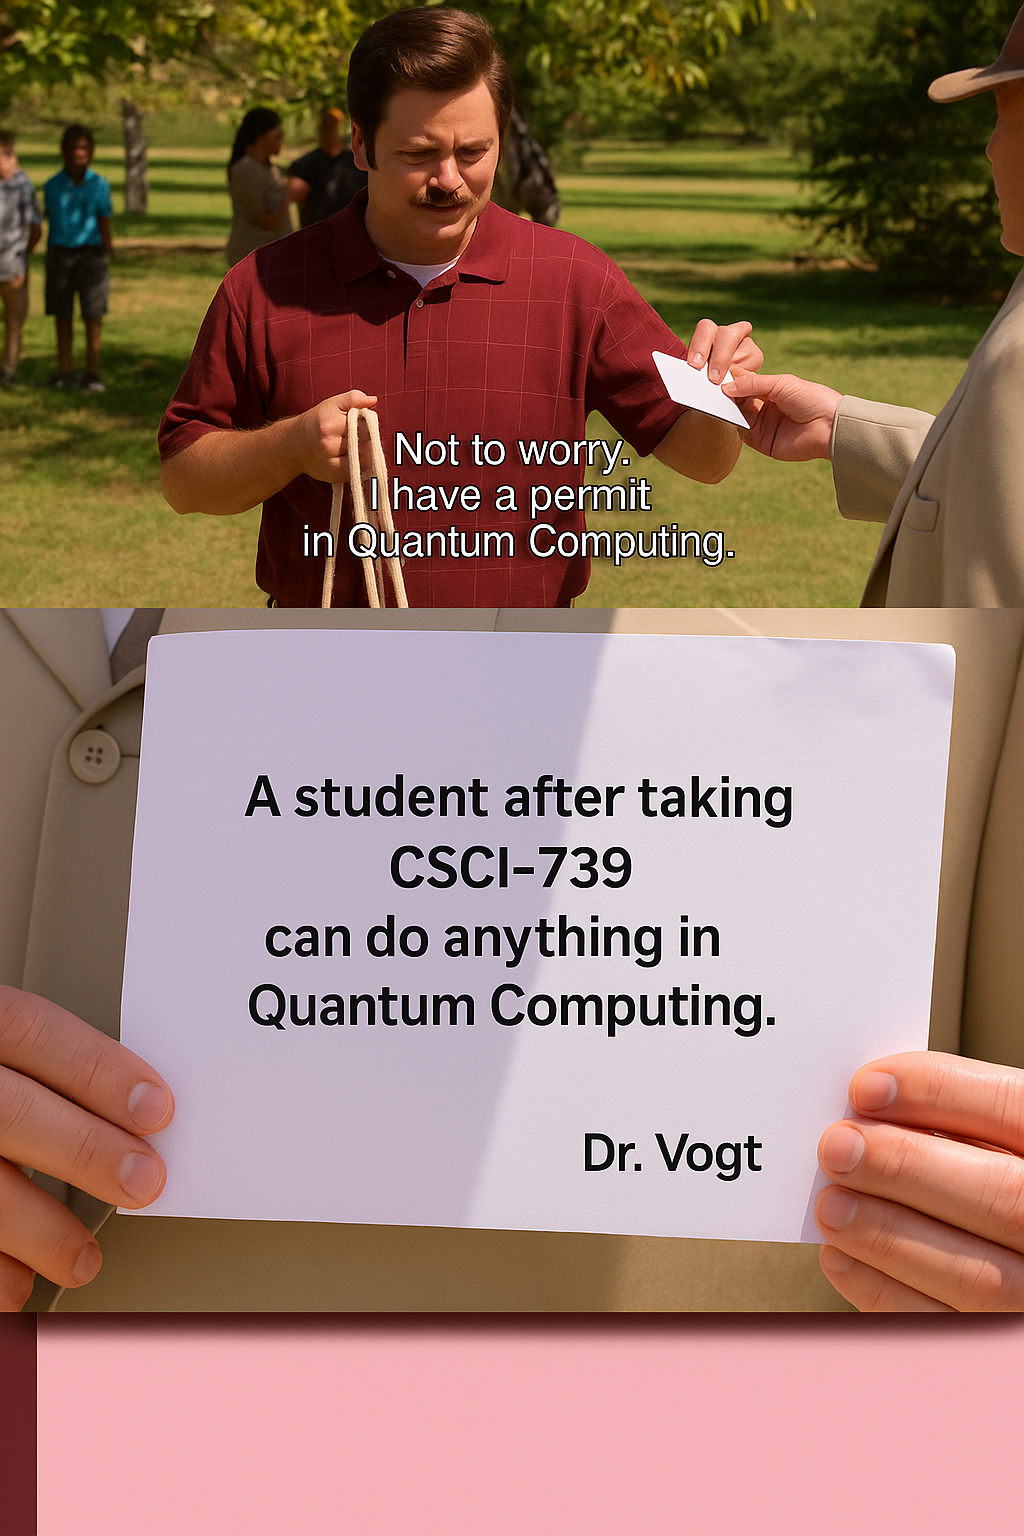
\includegraphics[width=0.75\textwidth]{quantumvogt3.png}
\vspace{0.5em}
\end{figure}

\newpage
\vspace{1em}

\noindent \textbf{Instructions.}  
For each paper listed below:
\begin{itemize}
    \item Read the assigned sections.
    \item Write a clear summary (1--2 paragraphs).
    \item Give your general takeaways and thoughts (3--5 bullet points).
\end{itemize}

This homework is optional, but strongly recommended for students interested in research, graduate school, or future work in quantum computing. Have fun! \smiley{}

\newpage

% ----------------------------------------------------------
\section*{Paper 1 — Quantum Approximate Optimization Algorithm (QAOA) \\
\small{(QAOA.pdf)}}

\begin{summary}
QAOA is a variational quantum algorithm designed to solve combinatorial optimization problems by alternating between cost and mixing operators.
\end{summary}

\paragraph{Connection to my research.}
I like to think about how quantum computers can impact \textbf{optimization theory}, which is deeply connected to \textbf{machine learning}. Optimization is everywhere in ML, and QAOA is a core quantum approach to these problems. \smiley{}

\vspace{0.5em}
\noindent\textbf{Your task:}  
Read the paper and write:
\begin{itemize}
    \item A 1--2 paragraph summary.
    \item 3--5 bullet-point takeaways or thoughts.
\end{itemize}

\newpage

% ----------------------------------------------------------
\section*{Paper 2 — Quantum PDE / Quantum Algorithms for Applied Mathematics \\
\small{(QuantumPDE.pdf)}}

\begin{summary}
This paper explores how quantum algorithms might accelerate numerical PDE solvers.
\end{summary}

\paragraph{Connection to my research.}
I am interested in how quantum computing may influence \textbf{applied mathematics} in general—PDEs, optimization, control, uncertainty quantification, and scientific computing. This paper gives a window into the future of \textbf{quantum scientific computing}. \smiley{}

\vspace{0.5em}
\noindent\textbf{Your task:}  
Read the paper and write:
\begin{itemize}
    \item A 1--2 paragraph summary.
    \item 3--5 bullet-point takeaways or thoughts.
\end{itemize}

\newpage

% ----------------------------------------------------------
\section*{Paper 3 — High-Fidelity Qubit Control and Pulse Engineering \\
\small{(QubitControl.pdf)}}

\begin{summary}
This paper analyzes pulse engineering and optimal control methods for producing high-fidelity quantum gates resilient to noise and hardware imperfections.
\end{summary}

\paragraph{Connection to my research.}
I am very interested in achieving more \textbf{stable quantum computation} through improved qubit control.  
There is also a \textbf{nascent effort} to explore whether ideas from this paper (originally for superconducting qubits) can be adapted to RIT’s \textbf{photonic quantum computing testbed} for running QAOA circuits. \smiley{}

\vspace{0.5em}
\noindent\textbf{Your task:}  
Read the paper and write:
\begin{itemize}
    \item A 1--2 paragraph summary.
    \item 3--5 bullet-point takeaways or thoughts.
\end{itemize}

\newpage

% ----------------------------------------------------------
\section*{Paper 4 — Decoded Quantum Interferometry (DQI) \\
\small{(DQI.pdf)}}

\begin{summary}
DQI is a quantum algorithm that frames combinatorial optimization problems as decoding tasks, using the QFT, structured quantum states (such as Dicke states), and constructive interference to amplify good solutions.
\end{summary}
\paragraph{Connection to my research.}
I am especially interested in exploring how the DQI algorithm can be applied to major, real-world problems in combinatorial optimization. Even discovering a way to effectively use DQI on just one high-impact combinatorial optimization task—for instance, a specific form of the traveling salesman problem—would already represent a substantial breakthrough. \smiley{}

\paragraph{Reading instructions (Important).}
The DQI paper is \textbf{80+ pages}.  
You do \textbf{NOT} need to read the entire paper (unless you really want to \smiley{}).

Please read only the following:
\begin{itemize}
    \item Abstract  
    \item Introduction  
    \item The illustrative max-XORSAT example  
    \item Figure 1 and the explanation of the 5-step DQI algorithm  
    \item The high-level discussion of the decoder  
    \item The semicircle-law intuition (conceptual level only)
\end{itemize}

This subset is enough to understand the core idea. \smiley{}

\vspace{0.5em}
\noindent\textbf{Your task:}  
Read the assigned sections and write:
\begin{itemize}
    \item A 1--2 paragraph summary of the DQI algorithm.
    \item 3--5 bullet-point takeaways or thoughts.
\end{itemize}

\newpage

% ----------------------------------------------------------
\section*{Final Reflection}

If you are ever interested in a capstone or research experience in quantum computing, feel free to reach out at rhvvcs@rit.edu. While these are some examples of projects I am currently pursuing, that doesn't mean I wouldn't be happy to oversee different quantum computing-related projects. If you have an idea and or an interest, I'm happy to mentor you regardless \smiley{}.


\end{document}
